
Salí al viaje por Bolivia y Perú luego de casi terminar de compaginar este
libro. Desde ahí envié mails contando el viaje a conocidos de distintas áreas
(trabajo, amigos, familia cercana y lejana), dirigiéndome con tanta cercanía
como la variedad de personas me permitía. También tenía en cuenta el entonces
proyecto de libro, para el que también escribía.

Mis familiares notaron un cambio de discurso en estos relatos, se lo atribuían
al gran viaje por dos países de Latinoamérica. Entre agradecimientos
contestaba que el cambio se debía más bien al estudio de mis relatos
anteriores y modo de vivir cada viaje, a un aprendizaje de mí mismo más que de
estos nuevos países.

La familia de mis compañeros (Eugenio y Guido), cuando llegamos, me preguntó
cómo había sido nuestra convivencia, cómo había salido el viaje (salimos
casi sin conocernos, ya contaré la historia). Y contesté que todo ese año
2008 rumiaría tantas experiencias y que, mientras tanto, sí que estaba muy
feliz.

Y así encontré otro placer en escribir mis viajes. El revivir los momentos ya
vividos, repensarlos, y continuar aprendiendo y seguir creciendo y disfrutando
aún después del viaje. Si viví Bolivia de una manera fue gracias a lo
aprendido en otros viajes y sus escritos; si aprendo del viaje también
participan las personas con quienes me relacioné y estos relatos.

Mi amigo Ezequiel había decidido no viajar en bici ese verano, y volver al
Noroeste Argentino con otros amigos nuestros. Me invitaron, pero preferí
conocer lugares nuevos, si bien aún no tenía planes definidos.

Un fin de semana nos visitaron unos amigos de mis padres de Rosario, entre otras
cosas nos contaron que sus hijos deseaban conocer Bolivia y Perú, y me
invitaban a unirme. Mis viejos conocían a estos dos hermanos, y los cuatro
``adultos'' me decían con entusiasmo que tendríamos gran afinidad, y les
parecía una buena idea que viajáramos juntos.

Mi pasaporte estaba aún en regla, decidí entonces unirme a los chicos en
conocer nuevos países. Un fin de semana de Diciembre viajaba a Rosario para
comprar el pasaje, pensando en tomar primero una cerveza con ellos, conocerlos,
evaluar la amistad y el viaje que podríamos lograr, y en base al supuesto
encuentro decidir o no la salida juntos. Pero nos encontramos en la Terminal
(les describí por teléfono cómo estaba vestido para reconocernos), y casi
nuestro primer cruce de palabras se ocupó de la decisión (a la que me
participaban, si bien me unía a un viaje ya en teoría planeado) de en qué
empresa viajar, y si llegar primero a Jujuy o directamente a La Quiaca. Fue
sorpresivo, pero desde esa primer encuentro encontré afinidad y comodidad.
Compramos pasaje en ``El Rápido'' hasta Jujuy. Y después fuimos a tomar una
buena cerveza al río.

\section{El altiplano boliviano}

\subsection*{5 de Enero -- Uyuni}

¡Hola, queridos! ¿Cómo andan? Por aquí todo de
lujo. ¡Me refiero a que está todo bien, nada más!

Después de treinta horas de viaje llegamos a La Quiaca, dormimos bien, y
caminamos hasta la frontera. En el Hospital me pusieron gratuitamente la vacuna
contra la Fiebre Amarilla, todo un alivio, el trámite inconcluso que traía
atragantado.

Cambiamos a pesos bolivianos en Villazón (Bolivia), y preguntamos por
colectivos a Uyuni, para visitar el Salar. Nos contaron que no hay ruta hasta
ahí, así que nos mandaron (en un proceso bastante desordenado) en un colectivo
hacia Tupiza, que queda camino a Uyuni. ¡Y la ruta desde
Villazón a Tupiza es de feo ripio! ¡Los colectivos son
altísimos, casi todo terreno, porque no hay caminos! Primera sorpresa.

Tupiza nos pareció un poco feo, y, luego de unas cuantas idas y venidas
(incluida la organización de 35 mochileros para contratar un bus), terminamos
contratando una Toyota Land Cruiser de los 80'\ para que nos lleve a la ciudad
del gran Salar. El viaje fue impresionante. Eramos nueve: tres bolivianos que
necesitaban viajar (y pagaron el precio ``turista'' porque sino tendrían que
esperar días a la salida del colectivo), nosotros tres (Eugenio Siri, Guido
Siri y yo), un cuarto argentino de San Antonio de Areco, el conductor y un amigo
suyo. Tres filas de tres, en un vehículo que se movía --no exagero-- como una
montaña rusa. El conductor conocía tanto al camino (sin contar los constantes
imprevistos) como a la camioneta.

Para completar los 210~km estuvimos seis o siete horas de puro todo terreno,
bien safari. Ruta de roto ripio, muchas veces siguiendo el cauce del río, al
principio bajo una lluvia torrencial (hasta adentro de la camioneta se llovía),
a veces cruzando vados grandes\ldots\ Las sorpresas durante el camino fueron
muchas (y sus correspondientes frenazos), no entiendo cómo algunos eligen
circularla de noche\protect\footnote{Todos los que recorrieron esta ruta de
noche en colectivo (charlamos con cinco personas, de tres grupos de amigos
diferentes) terminaron ``shockeados'', seguros de no querer repetir la
experiencia.}. Todas son camionetas de este estilo: todo terreno agresivo, pero
viejo. Sin embargo no vi Land Rovers, como las hay tanto por nuestro Sur. Los
bolsos viajan en el techo, junto con las ruedas de auxilio. En el camino
limpiamos el filtro de combustible, el conductor instaló \emph{un}
limpiaparabrisas porque habíamos salido sin, y cerramos una puerta con un nylon
en el medio para que no se lloviera tanto. Faltaba un tigre merodeando y
estábamos en 'Africa. Al principio selvático, luego paisaje del altiplano,
más árido y seco.

Casi chocamos, en un momento de casi nula visibilidad, con otra camioneta que
iba bastante rápido. Entre vidrios empañados y mal-limpiados, apareció una
(en dirección perpendicular en frente nuestro) tan rápido como desapareció.
``¡Casi vemos la luz!'' decía el conductor, entre nervioso y
gracioso. Nosotros contestamos que casi nos encandilamos con ``la luz'', entre
nerviosos y graciosos.

Cruzamos varias minas, y rondamos los 4000msnm. En La Quiaca me sentí débil y
mal, pero después me acostubré al aire enrarecido. Conocimos un pueblo minero
llamado Atocha, las casas forman desprolijas gradas cayendo de la montaña. Muy
histórico todo. Hay muchas esculturas a mineros, trabajadores y madres, por
todos lados. En La Quiaca en un monumento comparan a la mujer con Dios, por el
gran amor que tienen y dan, o algo así.

Uyuni es el primer pueblo que parece más bonito, llegamos y comimos en un lugar
de lugareños, pollo frito con papas fritas. Pa'\ engañá'\ al estómago.
Recién llegado y un poco cansado, me di el primer baño del viaje (a pesar del
agua \emph{congelada}), y a dormir, que mañana vamos tempranísimo al salar
para ver ahí el amanecer.

Los bolivianos conocidos son todos unos grandes. Lo del regateo que tanto se
habla parece verdad, pero nunca nos estafaron (Eugenio Siri se dedica a regatear
todos los precios). Estos de las Toyota tienen muy buena onda, y cobran
relativamente barato, mañana nos llevan al salar porque los volvimos a elegir.
Los tres bolivianos que nos acompañaron a Uyuni nos dieron la plata del viaje
a nosotros (unos \$100{\small AR} cada uno) para que arreglemos con el de
la camioneta, mucha confianza sobre completos desconocidos. Y con los Siri nos
llevamos muy bien, muy buena onda.

Mañana vamos a la tarde para Potosí, esta carrera es peor que las mías en
bici. Sin embargo conocemos mucho (y dormimos poco).

¡Un abrazo grande, y un beso grande a quien corresponda!

Tute.

\subsection*{6 de Enero -- Potosí}

¡Hola, queridos! ¿Cómo andan?

Ayer al amanecer fuimos a la mañana al salar en las Toyota. Como había
llovido tenía una capa de agua de 5cm, quietita como estatua reflejaba
perfectamente lo que hubiera sobre sí misma. ¡La camioneta
andaba sobre el cielo y las nubes! Leí que estar en el salar en una noche
estrellada lo hace sentir a uno en una nave espacial, ya que todo lo visible
está cubierto por estrellas, y pensé entonces: ``¡qué
`fumones'!'' Pero realmente se siente así. Las montañas en ese paisaje
crecen para arriba y también para abajo. Alucinante.

Conocimos el Hotel de sal, publicitado por la Secretaría de Turismo de Bolivia.
Era un desastre, atendido por un inexpresivo joven boliviano, que estaba más
quieto que el agua del salar. Los cables colgaban de los techos, los adornos
estaban desordenados, el ``museo'' parecía un engaño\ldots\ Podría ser un
lugar mágico, único en el mundo, pero ahora está descuidado.

El de nuestra Toyota estaba muy de acuerdo con Evo Morales y veía muuy
positivamente el estado del país; los muchachos de la otra Toyota nos contaron
que el conductor estaba en desacuerdo con Evo. El único que mencionó el
conflicto con Bolivia Oriental fue el primero, quien no emitió opinión
concreta, y no cree que se separen\protect\footnote{Referencia al conflicto
detonado semanas antes, cuando hubo dos muertos por cruces entre dos partidos
políticos opuestos, cuando Evo aprobó una Constitución sin presencia de la
oposición, según lo que leí.}. El hotel de sal tenía la foto presidencial de
Evo, pero le habían agregado por computadora la bandera indígena al lado de la
boliviana. De no creer.

Volvimos a la ciudad de Uyuni, almorzamos carne de llama, pedimos unos cafecitos
y trajeron tazas de desayuno llenas. Al terminar los cafés --aproximadamente
dos horas después-- caminamos al Cementerio Ferroviario, donde hay miles de
toneladas de hierro oxidado y retorcido, abandonados sobre las vías. Había
varias locomotoras a vapor antiguas, enormes; y muchos vagones y ejes. Los
durmientes son de hierro, no madera. ``Parece --decía Guido-- que les sobra el
metal, los tiran en lugar de volver a fundir''.

Tomamos unas cervezas en este día gris en un barcito, con otros grupos
mochileros. El contraste con los viajes en bici es notable. En bici se vive más
``ermitaño'', con mucho tiempo en silencio y de ejercicio, y mucha menos vida
social. De mochila se vive de modo mucho más social, y para estar en silencio
hay que buscarlo. Los dos estilos de viaje son igualmente excelentes,
invalorables y por eso incomparables.

Saldríamos a las 18hs hacia Potosí, pero las lluvias no permitieron llegar a
la Terminal al colectivo de nuestra empresa. Preguntamos en otra empresa si
tenían lugar y nos dijo la señora que sí, pero que seguro se quedaría
varado en la noche en el camino y nos moriríamos de frío; más valía
quedarse. Sincera la buena mujer. Rutas asfaltadas es lo que extrañamos.
Volvimos a otro hostal, un poco cabizbajos y con poco por hacer, pero salimos a
tomar cervezas con unas chicas de pueblo cercano a Pergamino, estudiantes de
Medicina en Buenos Aires, una más grande que la otra, interesantes en su
cerebro. Charlamos sin parar, hasta que llegaba la medianoche, hora en que
cierra el hostal. Quienes atienden tienen una hermosa buena onda, los chistes
van y vienen y no paran de trabajar.\\

A las 8 de la mañana salimos (esta vez sí) en cole a Potosí. Por el camino
subía gente hasta que, por falta de lugar, tuve que viajar con el bolso de uno
sobre mis rodillas. Llegamos luego de seis horas de recorrer paisajes
altísimos, por un camino impactante de alta montaña, de una mano y ripio, muy
parecido al de Iruya. Cruzamos varios camiones cisterna, otros que llevan
grandes máquinas mineras, varios colectivos y 4$\times$4\ldots\ imaginen la
velocidad a la que se circula.

Llegamos a Potosí, y nos asustamos un poco: se veía muy pobre, fea y
aglomerada, y con poca bienvenida turística. Cruzando la desprolija calle,
recién colgadas las mochilas a las espaldas, vi cómo una combi casi choca al
auto que tenía adelante; crucé corriendo sin entender la maniobra. El auto le
dejó lugar, y la combi empezó a escapar mientras dos tipos la perseguían
gritando: ``¡¡PARENLA, FRENENLA!! \textexclamdown
¡CRUZATE, CRUZATE!! (a un auto que había de frente)''. La
estaban robando. La camioneta y los dos bolivianos desaparecieron por una calle.

Nerviosos y callados, empezamos a subir para el otro lado, a 50 metros
encontramos dos tranquilos policías. ¿No se habrán enterado?
Nos indicaron el centro, diez cuadras hacia arriba. Caminando a arriba paramos
dos veces a tomar aire, el corazón acelerado nos muestra los 4000msnm a los que
lo hacemos trabajar. Llegamos a un hermosísimo centro. En info turística nos
hablaron con mucho placer de las minas y el volcán con aguas termales, del que
se desconoce la profundidad. Preguntré si las minas están en uso, a lo que
contestó que sí: ``¡Trabajan 9.000 obreros!''

Por \$10{\small AR} (pero en otra empresa, bienvenido Euge Siri
organizando) lo llevan a uno en minibus a las minas con trajes de minero, y lo
hacen entrar mientras trabajan. Uno puede aprender de los obreros, charlar, y
hasta trabajar con ellos (¡!). El salario de minero se debe
componer en buena parte del turismo. A europeos cobran \geneuronarrow{10}, unos
\$40{\small AR}, alrededor de \$80{\small BO}; con estos clientes
en mente otra empresa turística nos hechó antipáticamente de sus oficinas.

Aquí se nota más crudamente la diferencia rico/pobre: el centro (de estilo muy
colonial) no tiene nada que ver con el barrio donde bajamos del bus. Circulan
nuevas Mitsubishi al lado de destartalados taxis. El mercado de carne no tiene
refrigeración. Hay casi indígenas vendiendo pan casero en puertas de casas de
financiamiento. Hay cientos de abogados y dentistas. Vimos un sucio cartel
promocionando un cirujano, y una oficina de Ingeniería Civil. La Universidad de
Potosí es la más antigua de Bolivia.

Tenemos hambre: ayer no salimos a comer para ahorrar, y no cocinamos por vagos.
Hoy desayunamos mate y galletitas, y no almorzamos en el pueblo que nos sugería
el colectivero. En el centro potosino no encontramos ni un puto restaurantito
mochilero (los Domingos no abren estos chiringuitos), ni siquiera había
tamales. Decidimos esperar hasta el anochecer, para que se justifique pagar un
restaurant. ¡Los chicos se quejaban de que soy medio ciruja, pero
la ``cirujearon'' de lo lindo recorriendo restaurantes! Muchos abogados en
Potosí, pero pocos cocineros.

Dormimos en un ex-convento bicentenario muy lujoso, que raramente es hostal
mochilero, el ``Compañía de Jesús''. Los dueños, divinos. Hay ostentosos y
grandes edificios católicos por todo el centro. Sin embargo, en las minas creen
en ``el Tío'', el dueño de los minerales. Mañana lo conoceré.

Eso será todo por ahora. ¡Un abrazo grande a todos!

Tute.

\subsection*{9 de Enero -- Potosí y Sucre}

¡Hola, queridos! Muchas gracias por sus mails. Vine muerto de
cansancio seguro de que no escribiría, pero siempre lo mismo. Gracias de
verdad. Me alegran mucho todas las buenas noticias.

Ayer a la mañana fuimos a las Minas, al Cerro Rico de Potosí. Subimos en un
cole de línea, nos disfrazaron de mineros, y nos bajamos en un mirador. Nos
daba un poco de verg\"uencita bajarnos --turistas disfrazados-- mientras la
gente entra a envenenarse y trabajar hasta el cansancio por un pequeño jornal;
creíamos que los trajes no tenían sentido.

La esperanza de vida de los mineros es de alrededor de 45 años, al escucharlo
se nos atragantó la saliva. Los minerales, luego de separados de la piedra, son
enviados a Bélgica (para armamento) y Japón (para fotografía), entre otros
lugares. La guía es hija y nieta de mineros. Hoy le hicieron una multa, por
llevar tres turistas más de los permitidos por guía (11). Irónicamente se le
perdieron tres antes de entrar (por no esperarlos) que por suerte consiguieron
otro guía y no se perdieron la experiencia. En el mirador hicieron explotar
dinamita, el eco se sintió tres veces en el valle. Y entramos en la mina.

La pequeñita puerta daba miedo. La atravesamos y caminamos sobre una vieja e
inundada vía, agachados, siguiendo la única luz de nuestras linternitas, nunca
suficiente. Tomamos un desvío y bajamos por una escalera vertical que me
asustó un poquín. Mientras esperaba que bajen los compañeros vi pasar un
minero empujando una pesada manguera por el camino de la entrada. Después de
otras escaleras y caminar por ahí otro rato, bajamos por un ``tobogán'': una
caída cilíndrica de piedras, del tamaño de un cuerpo humano flaco. Había
que arrastrarse sobre el movedizo y húmedo suelo para llegar al tercer nivel
bajo la entrada, pero contra la pared derecha porque a la izquierda había un
respetable pozo. Volviendo a subir, para sortear el tobogán tuvimos que usar
las uñas y mucha fuerza, y las piedras de quienes iban adelante golpeaban a
los de abajo. Escribo todos estos detalles porque me sorprende lo rústico y
riesgoso del tour, poco ``turístico'' en el sentido grande del término. Al
principio daba mucha claustrofobia, luego se pasa. El ``inútil'' disfraz quedó
completamente embarrado, tenía piedras y agua en las botas. El ``inútil''
casquito amarillo me salvó de varios golpes contra los tirantes del techo, que
cada uno cruza a distinta altura. ¡El golpe seco mareaba!

Ya en el camino principal encontramos unos obreros que subían y bajaban un gran
balde mediante una polea, desagotando los niveles bajos de la mina. Por eso el
agua en las vías. Charlamos un rato, nos contaban que les pagan casi
\$100{\small BO} (una cena de restaurant sale \$30, una buena empanada
sale \$1, un viaje en colectivo sale \$1) si sacan dos vagoncitos de
piedras/piedras-preciosas por día, tarea que casi siempre logran. Les dejamos
las provisiones que la guía sugirió les compremos (gaseosas, cigarrillos,
hojas de coca, ``alcohol potable'' a 85$^\circ$). Estos chicos eran muy
jóvenes. Acá trabajan hombres, niños ({\small ONG}s de Alemania e
Italia invierten en su educación) y también mujeres (quienes separan los
minerales). El trabajo en la mina es casi obligado para los ciudadanos, no
tienen un abanico de posibilidades para elegir.\\

Bajamos con todo el olor de los minerales a la ciudad de Potosí, y recorrimos
el Museo de Santa Teresa. Esto era un convento de las monjas Carmelitas del
siglo {\small XVII} (ahora mudadas al edificio vecino para permitir la
apertura del museo). En la época, la decisión era muy social, no tan
religiosa: allí asistían pocas hijas de aristócratas españoles. Estos
podían comprar indulgencias mediante regalos a la Iglesia, por eso el museo
goza de una cantidad de arte y piedras preciosas. Me dejó picando varias ideas
que tengo que aún rumiar. Estos aristócratas, si había lugar en el convento
--para 22 monjas, que pasaban allí toda su vida-- dejaban a su segunda hija (el
primogénito era heredero, el segundo era para Dios) a los quince años en el
convento, y ya nunca más las podían volver a ver (ahora no es tan cerrado). Su
educación en la niñez era religiosa, y luego adoptaban votos de castidad y
humildad. Si bien ahora es tan ostentoso porque es museo, ellas vivían allí
una vida más sencilla. Su carisma era y es la Oración. Pero qué se yo\ldots\
creo en esta religión y sin embargo no me sentí en mi salsa. Ellas vestían a
Jesús y María con todas las pompas, yo los imagino muchísimo más simples
(que no es más que la descripción de los Evangelios). Conozco un sacerdote de
este estilo: a él le regalan ropas y cosas para mejorar su nivel de vida, pero
él está contento como vive. Vuelve a regalar lo que regalan, y continúa
vistiendo sus ``viejas'' camisas. Simple y llana humildad, con eso comulgo más.
Pero en fin, cada uno con su carisma.

Cenamos unas flacas empanadas en la peatonal (triste estafa la gordura que
ostentaban), y vimos pasar 4 veces a los mismos 50 habitantes del Centro: la
vuelta al perro parece ser. Y a dormir.

Fuimos esta madrugada a Sucre, recorrimos la primer ruta asfaltada del viaje por
Bolivia. La entrada al pueblo se hizo larga entre muchas construcciones
precarias, luego llegamos al centro colonial que tiene viejas y hermosas
construcciones. Caminamos mucho, todo nos impresionó. Visitamos la Casa de la
Libertad, donde se declaró la Independencia boliviana, un lugar emocionante
(hubo mucha participación argentina). Néstor (Kirchner) colgó una placa con
su nombre grande frente a una que nombra a Belgrano, saludando al pueblo
Boliviano en un aniversario. No incluye a ningún otro argentino más que a este
Kirchner, todos los turistas argentinos mostramos sonrisa molesta. En 2009 se
cumplen 200 años de esta Declaración, los festejos se vienen a lo grande
(igual que en 1909).

Luego visitamos el Museo Folklórico, cuyo objetivo es mostrar las comunidades
indígenas que actualmente viven cerca de Uyuni con sus costumbres ancestrales.
Es gratuito, bien por Sucre. Un extranjero no podía cerrar su boca cuando le
hicieron entender que sí, que esas fotos que parecen ilustraciones
enciclopédicas son actuales. Una larga sala era dedicada a caretas
carnavalescas, la alegrísima y autóctona música de fondo invita a quedarse
también en Febrero. ¡Quedará para 2009, junto al bicentenario!

Sucre presenta mucha evidencia de las últimas manifestaciones. El cuartel de
policía fue saqueado: tiene prendida fuego una puerta y otra rota, todos los
vidrios rotos, y algunos graffitis xenófobos y contra Evo. El edificio de
Prefectura también tenía vidrios rotos. Acá se nota más el caldo caliente
que tiene que gobernar el pobre Evo\ldots\ odio entre los mismos conciudadanos
muestran los graffittis, no se si serán tres locos o un porcentaje
significativo de Bolivia.

También vimos bastante pobreza de emergencia: gente avejentada con cara de
hambre mendigando pocas monedas. La pobreza anterior es ``digna'', en el sentido
de que tienen llamas o empanadas para comer, y una lata o pajas bajo las cuales
reposar. Un grupo de revoltosos niños morían por lustrar nuestras embarradas
zapatillas, negociamos en cuatro paquetes de galletitas para los seis, sin
lustre. Tuvimos que darles unos tirones de orejas para que las compartieran.
Pregunté a una señora por direcciones de lugares, y me contestó que no
entiende lo que digo: sólo habla Quechua.

A las 18hs salía nuestro bus, así que en taxi conocimos la Recoleta, un
selecto barrio sobre un cerro, con vista panorámica a toda la ciudad. Después
fuimos a la terminal. Nos restó otro día para conocer diversas Iglesias (hay
una cada dos cuadras) y el histórico Cementerio; ¡para 2009!

Un beso muy grande a todos;

Tute.

\subsection*{10 de Enero -- La Paz}

¡Hola, queridos! ¿Cómo andan?

Ayer a la mañana fuimos a la Casa de Moneda de Potosí. Mostraron la parte
técnica de cómo los españoles hacían sus monedas con minerales del Cerro
Rico, cómo las transportaban en complejas cajas fuertes, por dónde las
llevaban al mar y a Europa, etc. Dicen que la riqueza que salió de aquí hacia
España es más grande que la de Tutankamón, y la comparaban con la de otro
reino. Un barco con cajas fuertes provenientes de aquí se hundió cerca de
Miami, lo encontraron hace poco. Nuestras monedas de un peso argentino conservan
el histórico logo PS (``Potosí'', solapado de un modo raro), por algo
relacionado con Belgrano que no recuerdo. También hablaron de la ironía de que
los billetes bolivianos se produzcan ahora en España. Mundo loco.

¡Me entreré en la Casa de la Libertad, en Sucre, que nuestra
bandera tenía celeste en el medio y blanco en los costados! Estos colores
corresponden a la casa de Borbón, Belgrano era promonárquico. Y yo me tragué
el sapo de los colores del cielo; qué verg\"uenza, maestros de primaria y
escuelas argentinas. A los niños no les surje pensar en la casa de Borbón a
los diez años, pero podrían mandar otro sapo menos na\"ive, y enseñar algo
más real en años posteriores.

Fuimos a la iglesia de San Francisco, conocimos sus catacumbas y una increíble
vista panorámica a Potosí. Imaginen subir al techo (literalmente, a las tejas)
de una gran iglesia, para mirar desde allí (ya arriba de una montaña) al
pueblo y valle.

Conseguimos pasajes para esa noche a La Paz, vía Oruro por falta de lugar; un
viaje cansador. Y utilizamos las horas que restaban tomando un bus a Tarapaya.
La ruta baja de los 4.200msnm a los 2.500msnm aproximadamente, por un valle
edénico. Si bien queríamos conocer un volcán con un lago de aguas termales en
su cráter, el bus nos dejó bajo una montaña, que tendríamos que trepar con
las mochilas. Luego de 20 minutos de cansancio llegamos a una primer pileta, de
alrededor de 45$^\circ$C. Después, otra que largaba humo y burbujas:
120$^\circ$C. Sí, quemaba. Al final, y luego de un morro, apareció el cráter
junto a un muy amigable y simple cuidador.

El hombre nos explicaba, con una paz oriental, que este piletón de 50m de
radio, lugar sagrado Inca, ``no tiene profundidad''. Nos permitía cruzarlo, y
de hecho nos aconsejaba hacerlo, a pesar de los rumores de remolinos y de
peligro. ``Lo que pasa --decía-- es que acá vino gente que no sabía nadar, o
se metieron borrachos. El único requisito para meterse es saber
nadar''. De todos modos creo que no prestó atención al posible gran cansancio
o relajación de los pampeanos, no creo que fuera peligroso pero tampoco
sencillo. Estaba completamente seguro el hombre de su fortuna, pues le toca
vivir en un lugar cercano al Paraíso. Se lamentó que no pasáramos la noche, y
nosotros también.

Este cráter envía desde su centro burbujas a modo de hidromasajes, y el agua
tiene una temperatura de 35$^\circ$C (en el centro más, en la periferia menos).
Uno hace la plancha y ve límpidos cielo y sol; o mira hacia adelante nadando y
ve el valle alejarse, creciendo desde abajo hacia arriba; o mira a los costados
y ve enorme y pura Cordillera de los Andes. Sí que es un lugar sagrado. Nadando
no pensaba en la literalmente inmensurable profundidad, al hacerlo me
desesperaría queriendo salir y perdería el aire. Guido fue el primero en
meterse: con un pie en la playa, puso el otro sobre el agua, y desapareció
instantáneamente. El cráter tiene paredes casi verticales.

A pesar de la increíble belleza no lo visita mucha gente, no sabemos porqué.
Pero lo hace más particular. Y nos fuimos casi corriendo a tomar el último
cole a Potosí, con mucha alegría nos despidió el hombre, invitándonos
--varias veces-- a volver. Le quedan 3 años de bonanza y paz, cuidando este
punto único del globo.

Y empezamos el viaje a La Paz. Llegamos cansados a la madrugada, conseguimos
gracias a amigos mochileros un increíble hotel cerca de la plaza central. Hotel
Torino, a media cuadra de la Plaza Murillo. La suerte en este viaje juega de
nuestro lado: lo que puede salir mal o bien, sale bien. Conseguir pasaje a La
Paz fue otro ejemplo. Llegar a tomar el último cole a Potosí (y no perder el
cole a Oruro), otro. Y así cuentan\ldots

Tomando vacaciones de las vacaciones dormí una buena siesta, y después salí a
caminar. Los chicos recorrieron durante mi siesta. Alrededor de esta plaza
central, además de la Catedral, Casa de Gobierno y otros edificios
institucionales, hay mercaditos como en cualquier galería barata porteña.
Sorprende. Otros edificios institucionales se reparten entre las cuadras de
alrededor. La Paz es muy linda en su centro, con casas coloniales históricas,
una buena peatonal, y calles relativamente ordenadas. Se siente la falta de
``cafetines de Buenos Aires'', entre el frío y el hambre que incitan a
buscarlos. El único que encontré en decenas de cuadras tiene vista a la calle
sólo a través de su vieja puerta.

Caminando, uno mira siguiendo una calle a la montaña lejana, y parece paisaje
típico cordillerano, pero lo extraño es que no se trata de una simple y
lejana montaña sino que está llena de construcciones. El centro de La Paz
presenta edificios, y las montañas que lo rodean también están cubiertas de
edificios. Un paisaje nuevo.

Así como en Sucre había graffitis y papeles exhibiendo firmes ``La Capital se
mueve'', en La Paz los carteles rezan ``La Capital no se mueve. En lucha por la
unidad.'' Oportunamente las monedas tienen grabado un ``La unión hace la
fuerza''. Si Evo Morales no visita el volcán de Tarapaya se queda pelado del
estrés en poco tiempo\ldots

Visitamos el Museo de Arte Nacional, estos muchachos me están enseñando a
mirar arte.

¡Un beso y un abrazo muy grande a todos!

Tute.

\subsection*{13 de Enero -- Coroico}

¡Hola a todos los queridos!

El 11 de Enero fuimos en la mañana a Tiwanaku, ruinas precolombinas cercanas a
La Paz. Aparte de muy interesante lo mostrado, el guía era muy buena onda, así
que la pasamos bien. Lo ``más'' de esta civilización preincaica: usaban
canales de agua para que la amplitud térmica de la tierra no fuera tan alta, y
poder así cultivarla. También, las construcciones, y el dominio de metales que
lograron. Hablaban Aymará, que dio forma al Quechua (Inka), junto con otro
dialecto.

Las dos noches en La Paz salimos a bailar, estuvo perfecto. A las 4am cierran
por ley todos los bares, y volvíamos a dormir.

Esa tarde contratamos un tour en bici por la ``ruta de la muerte'', que une La
Paz con Coroico, 64~km. Pasa por La Cumbre, donde llega a 4.700msnm, y baja
hasta los 1.200msnm: ¡3.500m por descender! Tiene el ancho
promedio de un camión, y es en su mayor parte de ripio. Está tendida sobre una
montaña muy escarpada, casi vertical, y recorre desde la inhóspita y nevada
Cordillera de los Andes hasta las verdes y húmedas Yungas bolivianas. En fin,
legendaria.

A las 6:45am nos levantó un guía, tienen los dos una buena onda fenomenal. Me
levanté cansado (con Euge dormimos dos horas) pero, todavía con la euforia de
ayer, no paré de hacer chistes, todo el día. Desayunamos juntos el grupo de
quince personas, y salimos en cole a ``La Cumbre'', el punto más alto de esta
ruta.

En el colectivo fui charlando con una de las aventureras: era estudiante de
Teología en G\"ottingen, que hizo un curso en Flores, Buenos Aires. El mundo es
un (increíble) pañuelo. Nos entregaron las buenas bicis más abajo de la
cumbre por la cantidad de nieve que había, ¡y a empezar! La
primer mitad por la ruta nueva, con autos y camiones pero ancha.

Se avanzaba naturalmente rápido, aunque aprendiendo el equilibrio de la
desconocida bici y frenando con cautela por lo mojado de la ruta. Muertos de
frío, veíamos a las montañas ``crecer'' a nuestro alrededor a medida que
bajábamos. Se iban tornando verdes, con innumerables y enormes cascadas
decorando todo el paisaje; la vista se turnaba entre el valle y la ruta. Se
sentían los vientos, las lluvias, las nieblas, las lloviznas, los olores\ldots\
todos distintos, todos en la cara. Los dedos sólo sentían frío.

Recorridos unos kilómetros, tomamos el desvío a la ruta vieja; fue la primera
vez en mi vida que sentí peligro en serio. Ibamos rápido por las piedras por
\emph{ese} camino: una piedra que descolocara hacia afuera al manubrio implicaba
instantánea y larga caída. Sin embargo era muy divertido. Cuando uno podía
olvidarse del precipicio y miraba al paisaje, al camino, y pedaleaba
frenando\ldots\ se divertía mucho. La mayor parte sabía que no iba a morir,
porque soy joven. ¿Cómo podría? Pero los escasos minutos que
sabía lo contrario se hacían largos y nerviosos, hacían difícil andar bien
en la bici. Por eso más valía olvidarse, y concentrarse en la diversión. Esto
deben hacer los que practican deportes de riesgo.

Hubo una parte increíble: a la derecha se levantaba una pared vertical de
decenas o cientos de metros, que se abría hacia afuera hasta pasarnos a modo de
techo. Y desde allá arriba se veían caer grandes cascadas, que formaban una
cortina de lluvia torrencial todo a nuestro lado. Ver las gotas ir cayendo por
el precipicio despacito, todas separadas, chocando al camino y cayendo al
profundo valle, emociona.

Había que hacer fuerza para accionar los frenos a disco, y con el frío de las
eventuales lluvias yungueras y el constante traqueteo del manubrio los dedos se
entumecían. Los descansos eran por eso necesarios.

Paramos a tomar algo en un mirador, mientras nos contaban la historia de esta
ruta: antes se cobraba hasta doscientes vidas al año. Ahora construyeron la
nueva, que tampoco es gran alivio: el suelo húmedo no ofrece sostén perfecto
para el asfalto, que a veces se derrumba. Han muerto ciclistas del modo más
estúpido: dejando lugar a un camión para que maniobre (exigen que sea del lado
del precipicio, para que los camiones que suben carguen con su peso la parte
interna de la ruta), y patinándose un poquito, para nunca más volver\ldots\ No
hay árboles que frenen: uno apoya un pie afuera y cae, como en el lago vertical
de Tarapaya. Lo irónico es que a veces perdíamos la atención del camino
pensando en lo peligroso que se veía el precipicio al costado, inquietante. La
invulnerabilidad y el miedo se interrumpían del mismo modo que en estas
líneas; era cuestión de divertirse, o andar con (pero sin) necesario cuidado.
O frenar y subir al bus.

Era cuestión de divertirse, los guías aquí se relajaron y nos contagiaron: la
ruta se tornaría desde allí más ancha, los precipicios serían menos
agresivos y con más vegetación; y, los que quisieran, podrían acelerar,
siempre que no adelantaran al primer guía. Un holandés, un peruano, el guía y
yo liderábamos, pasándonos entre nosotros, fue emocionante. Cruzando vados a
fondo, doblando todo lo que las piedras sueltas permitieran, frenando con fuerza
antes y durante las curvas\ldots\ todo terreno. Siempre el paisaje perfecto,
pero no teníamos mucho tiempo para poder verlo, sólo en paradas.

Y llegamos a Coroico, todos tomaron cervezas menos yo (continuando el chiste de
la resaca). Almorzamos, y tomamos sol en una pileta alta de Coroico, mirando al
enorme paisaje. Lo particular que tiene, lo que lo distingue de todo lo que
conozco, es que las selvas cubren montañas cordilleranas altas. Es como
Villavicencio (Mendoza) pero con la vegetación del Sur, o como el Sur pero con
las altas montañas mendocinas. (¡Conozco el Sur, Mendoza y
Bolivia como verán!) Y las rutas escapándose de esto como serpientes: la
vieja y la nueva tendidas sinuosamente sobre los accidentes grográficos.

Me acosté en un hostal de Coroico a las 21hs, ``un ratito'', y me levanté a
las 3am muerto de hambre. Un buen hombre me calmó con dos panes. Seguimos
durmiendo hasta las 9am.\\

Conocimos en La Paz a un alemán que está haciendo su servicio social
obligatorio: trabaja en El Alto, la parte pobre y lejana del centro paceño.
Fuera de esto, también ofrece facilidades via {\small ONG} a las
familias de numerosos niños lustrabotas de la Capital, en su tiempo libre
digamos. 20 años alemanes, uno acá conociendo la vida boliviana y sus
turistas, y vuelta a Alemania a empezar, probablemente, Ingeniería Civil. Una
cabeza grande.\\

Hoy visitamos una comunidad afro-boliviana cercana a Coroico, Tocaña. Los
trajeron para trabajar en las minas, pero los negros no se habituaban al frío y
a la altura; los bajaron entonces a estas Yungas para que cultiven coca y café.
Conservan pocas de sus costumbres africanas, entre ellas, un canto a la muerte
cuando muere un viejo casado. Son 35 familias ahora libres y dueñas de sus
plantaciones. Tienen todos una sonrisa enorme.

Adelantaron los Carnavales de Oruro: 2 y 3 de Febrero. Tenemos los ojos
desorbitados, con decirles que Guido va a llegar tarde a las primeras clases en
la facu. ¡No llegaremos de vuelta en Enero como creíamos!

Con los chicos decimos que Machu Picchu termina siendo para este viaje una
consecuencia, dado que cada día vivimos algo que justifica todo un viaje.
¡Cada día vivido acá justifica un viaje! Cuzco nos llegará
como un \emph{buen} postre. Y es que para vivir así, más vale no morirse
nunca. Estamos durmiendo poco por todo esto.

¡Un abrazo muy grande a todos! Muchas gracias por sus mails;

Tute.

\section{Lago Titicaca} \subsection*{16 de Enero -- Copacabana}

¡Hola, queridos! ¿Cómo andan?

Nosotros, antes de ayer en Coroico, hicimos una caminata por arriba en la
montaña --un buen sendero con constante vista panorámica-- para conocer tres
cascadas. Cinco horas estuvimos caminando, a Dios gracias que un minibus nos
acercó a la vuelta al pueblo. Sin querer seguimos semejante camino:
típicamente se usa el camino ancho y bajo de los autos. Pero, perdidos por
perdidos, seguimos caminando, y conocimos las cascadas casi desde donde nacen.
Dos brasileros que nos encontraron se volvieron en la segunda, no era fácil la
verdad. Euge incentivaba a estos dubitativos caminantes.\\

Esta tarde conocimos la ya mencionada colonia afro, en Tocaña. Conocimos ahí
al ``Pulga'', un antropólogo paceño y anarquista que vive ahí, y charlaba
interesante. Un muy buen tipo, nos hubiese encantado pasar la noche en su casa
junto a otros turistas pero ya habíamos contratado la vuelta, y teníamos los
equipos en Coroico. Todo no se puede, ¡siempre con sorpresas! Y
al siguiente día viajamos a Caranavi, un pueblito en las Yungas de Bolivia, por
la continuación de la ``ruta de la muerte'' pero sin el nombre turístico. Se
nos hizo largo el viaje, sin asiento entre tanto traqueteo.

La verdad es que era feo Caranavi, y parecíamos los únicos turistas. Con clima
lluvioso, salió una caminata para conocer el río, única actividad que
encontramos. Caminar por paisajes selváticos es bien placentero, si bien nos
mojábamos con la lluvia y los mosquitos me robaban la mitad de la sangre.
Encontramos por ahí a tres viajeros que ya habíamos cruzado en Coroico, y nos
sentamos a charlar un rato. Estaban en la misma que nosotros. Son una pareja
israelí, y un español que era un meo de la risa; todos haciendo largos viajes
latinoamericanos.

A las tres de la tarde empezó a llover de forma torrencial, así que nos
guarecimos tomando cervezas en un quincho que ellos conocían. A las 19 y luego
de unas cuantas cervezas surgió hacer un asado, la buena mujer nos permitió
usar su quinchito. Nos llamaba cariñosamente ``mis gringuitos'', y nos ayudaba
siempre que le pidiéramos (¡contadas veces, aparte de pedirle el
quincho!). Hicimos dos pollos asados y otra carne (bien asados, dada la falta de
refrigeración), y una ensalada tan grande que no logramos terminarla. El
español soñaba con esto desde que supo que somos argentinos, recordaba con
alegre melancolía el asado gratuito con que lo recibieron en su primera noche
en Buenos Aires. Dice que allá en España hay ``asados'', pero el circo
argentino es lo que lo hace sentir especial; esa espontaneidad y simpleza\ldots\
Ese ``¡Dale! Hoy asado en casa''. Lo escuchábamos sonrientes.

Todas las charlas eran de lo más interesantes. El israelí nos contaba que
allá no hay tanto lío como nosotros le describíamos, no se vive con miedo en
Tel-Aviv como yo imaginaba. ``Es más --decía-- si hoy un fundamentalista hace
explotar un colectivo lleno, mañana todos salimos a continuar nuestra vida
diaria y nos subimos a la misma línea de colectivos. Un par de locos no van a
detener nuestras vidas. No haremos como en Atocha, que la gente tenía miedo de
volver a salir.'' El español asentía.

Odia su servicio militar obligatorio de tres años. Luego de cumplir con esa
condena su Gobierno los puede llamar 40 días al año, siempre que les sean
necesarios al ejército. Su hermano ahora andaba disparando no sé dónde,
cumpliendo esta obligación. Triste. Sin embargo, contaba, hay judíos en el
exterior que viajan con gusto a Israel para cumplirlo: derramar su sangre para
defender el (¡por fin!) propio país les significa un gran
orgullo. Los israelíes tienen lío, según él, con fundamentalistas palestinos
(la Franja de Gaza recién tomada por Hammas creo). Y contaba también que en
todo alrededor de la dividida Palestina se ve mal a sus pobladores, sea por
parte de Israel, de Egipto, o de Irán (otro loco ese presidente).

En un momento David nombró un arma para darnos idea del tamaño, pero le
respondimos con cara de signo de pregunta. Entonces el español lo gastaba:

\subparagraph{}\label{ssub:israelies} --- ¿Han visto?
¡Estos tíos saben pollas de armas! -- a lo que ellos contestaron
casi a coro:\\ --- Ojalá no tuviéramos que aprender todas esas mierdas, pero
tenemos que hacerlo porque nos obligan. Ojalá no supiéramos disparar un arma.
Pero eso dicen todas las generaciones, nuestros padres dijeron esto, y es
siempre igual.\\ \hangindent=1cm

Contaba que cuando salió del liceo besó fervientemente el suelo y su libertad.
Desolador.

Luego nos hablaba con fanatismo del relativamente nuevo país: dice que al ser
una unión de judíos provenientes de cualquier punto de la Tierra, gozan de
muchas culturas y, por ejemplo, se jactaba de tener la mejor cocina y las
mejores mujeres del mundo. Comidas africanas, americanas, europeas, asiáticas;
lo mismo con las personas. Dice que es curioso pero común ver increíbles rusas
al lado de petisos marroquíes, parece que se gustan. Su novia moría de la
risa.

Durante el asado cayó un personaje de Caranavi, de unos 50 años. Dijo pocas
cosas, entre ellas que a él se le facilita hacerse amigo de los turistas porque
no los mira como a marcianos, como otros bolivianos (lo sentimos más de una
vez), sino que simplemente se sienta y charla. Nos invitó a dos cervezas
demostrando que no le interesaba si veníamos con plata o no (actitud opuesta a
muchos, realmente), y se fue. Un tipo simple, que participó poco de las charlas
religiosas.

El español enseña buceo en Barcelona, sus charlas se dividían entre
graciosas y técnicas, cuando le preguntábamos. Nosotros hablábamos de cómo
se vive tal o cual cosa que mencionábamos, en nuestras ciudades y país. Por
ejemplo, hablábamos de que estudiamos carreras, y la chica moría de envidia:
para poder estudiar idiomas ella tiene que hacer malabares con el trabajo,
porque la Universidad les es muy cara. Dado que sus viajes continúan por Chile
y Argentina, les recomendamos mucho por hacer y conocer.

El israelí, David, nos terminó contando del aparente hallazgo del cuerpo de
Jesús y sus ``discépolos'' en Jerusalén (tirando por la borda la Ascención
en cuerpo y alma del Mesías católico). Y empezamos a ordenar el quincho, para
volver a nuestros aposentos.

Un día fiero pintaba, pero salió un increíble encuentro. Besos a la dueña
del quinchito (irónicamente llamaba ``Jesús'' a David, porque se parece al
Jesús de las estampitas), y a medianoche volvimos a nuestros hostales.\\

Ayer pasamos un día completo viajando, para llegar a Copacabana. Imaginen estar
a alrededor de 4.000msnm, con un lago tan enorme frente a sus ojos que la vista
se pierde en el horizonte. Es como el glaciar Perito Moreno: uno puede sentarse
horas para mirarlo sin aburrirse. Y eso hicimos hoy, en el mirador de Copacabana
(hermosa ciudad), donde también leímos y conocimos gente. Las ciudades
costeras son mi debilidad, las amo por su olor a aguas, su gente generalmente
relajada caminando, sus platos de pescados frescos y baratos, y su --también
generalmente-- hermosura. Si es con montañas, mucho mejor. ¡Y
si es arriba, en la Cordillera de los Andes, ni les cuento!

\begin{center} 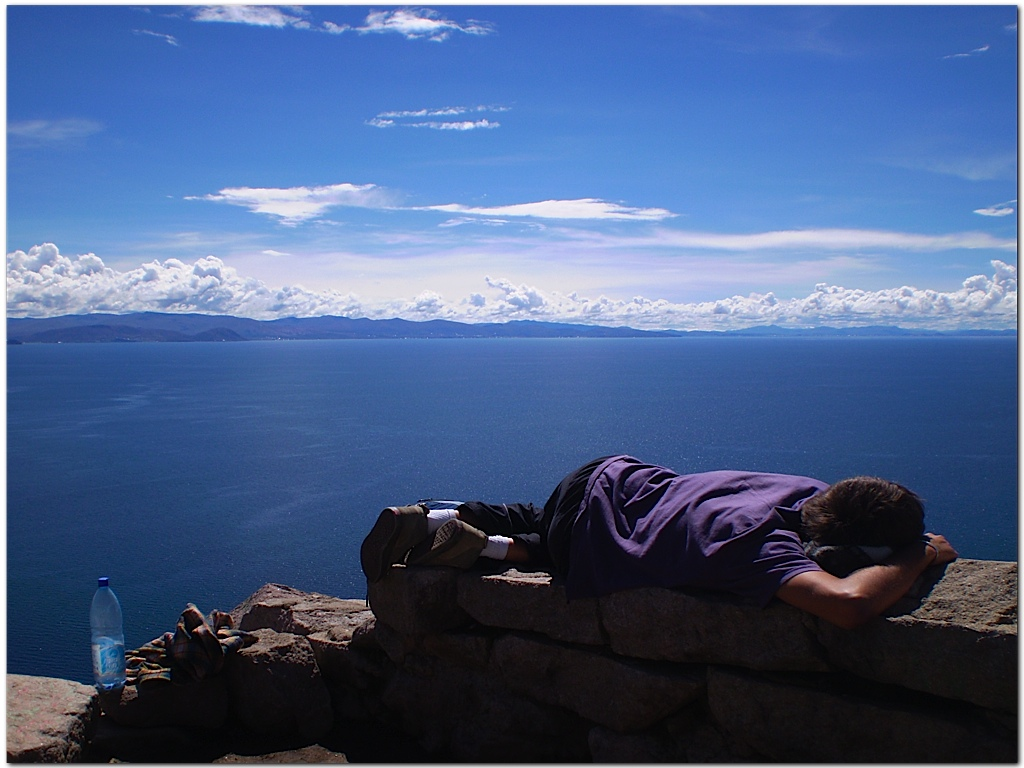
\includegraphics[width=300px]{images/P1160059.JPG} \textsc{\\Paz
en el lago.} \end{center}

Siempre que podemos desayunamos, almorzamos y cenamos en comedores municipales.
Son galpones llenos de mesitas (cada una correspondiente a cada cocinera), con
todos los precios iguales, informados en pizarrones colgados sobre la pared.
Viene más gente vaqueana del lugar que turismo, y nos encantan a pesar de la
nata de la leche.

Por Bolivia encontré común la imagen del Cristo completamente lastimado, luego
de los azotes. Es característico de este arte barroco-mestizo parece. Se le da
mucha bolilla al Cristo y la Virgen dolorosas, será por el pueblo oprimido
sobre el que instalaban esta Religión, tal vez. También vimos hoy muchas
ofrendas a la Pachamama. No me gustó que pedían todo material, pero nos
divertía ver la mezcla: tirando cerveza a la Madre Tierra, haciendo explotar
pirotecnia, con una cruz cristiana e incienso quemándose\ldots\ extraño, y un
toque milagrero. Pero vi otros devotos de la Pachamama que hablaban más,
digamos, a nuestro estilo (el de los chicos y yo): simple, y con amor y fe en el
centro.

¡Un beso enorme a todos!

Tute.

\subsection*{19 de Enero -- La Isla del Sol}

¡Hola, queridos! ¿Como andan? Este mail sale de
teclado norteamericano, en Perú. ¿Descuido o mucho turismo por
Cuzco?

Recorrimos Copacabana, la ciudad turística boliviana, lindante con el Lago
Titicaca. Divino. Comimos pescados más que pollos fritos por aquí, un placer.
Al otro día tomamos una lancha a la Isla del Sol.

La Isla del Sol es una islita montañosa de casi 20~km de largo por 8~km de
ancho. Se llega a su parte Norte luego de pagar \$15{\small BO}, y de unas dos o tres
horas de navegación. Es paradisíaca. Un nativo hizo de guía, llevándonos a
miradores y a las ruinas Incas que hay al Norte de la isla. Caminamos un buen
rato, y luego de unas charlas sobre su modo de vida e historia de la Isla, nos
describió el camino al Sur, donde descansaríamos y dormiríamos. Nos
despedimos, ya que él volvía a su pueblo, y nos sentamos un rato a descansar.

Como casi todos los días, en la mañana llovió, pero desde el mediodía
acompañó un buen sol. Desde este punto en que tomábamos mates se veían
varias playitas casi vírgenes, de arena clarita, agua azulada, y el lago y
otras islas cercanas. Quedábamos cinco viajeros, tres niños del lugar, y de
vez en cuando cruzaba algún pastor cuidando ovejas, no se porqué tan poquita
gente en tamaño lugar. Bajé a la playa para sentir el agua, daban ganas de
instalar una carpa y quedarse una semana de sereno ocio. El paisaje es perfecto,
las aves van y vienen, hay gran silencio interrumpido por ovejas, y rodean las
ruinas sobre la verde montaña. El agua es fresca, casi tan fría como la de
Mar del Plata; sólo molestan las algas del suelo. Huele un poco a mar, ya que
tiene muchos peces y es lago salado (se formó, como el Salar de Uyuni, a partir
un mar que cubría todo).

Subí fresco a donde me esperaban, y empezamos la caminata a la parte Sur. Cinco
horas de fuerte sol por la cresta de las montañas que dan forma, a la isla,
cansador pero perfecto. Cada ondulación significaba un increíble mirador al
Lago.

Ya en el Sur descansamos, leimos mirando el atardecer nublado y de vivos colores
celestes y rojos, cenamos bien, y a dormir, mucho. A las 5am nos levantamos para
ver si valía la pena salir a mirar el amanecer, pero estaba un poco nublado y
decidimos seguir durmiendo. El frío, ademas, es intenso cuando no hay sol.\\

Esa mañana (de ayer, 18) visitamos el Templo del Sol, casi en la punta sur de
la isla, y luego bajamos a una playita de rocas también casi virgen, donde nos
pasaría a buscar una lancha para volver a Copacabana (de película). A los 15
minutos apareció, subimos, y nos trajo de vuelta al pueblo, desde donde
empezaríamos el viaje a Perú.

Luego de trámites rápidos en la frontera, llegamos a la tarde a Puno, Perú.
Ahí visitamos a los Uros, una comunidad aborigen antigua distinta de los
Aymarás e Inkas. Ellos se instalaron literalmente en el Lago Titicaca, sobre
islas flotantes artificiales armadas a partir de la planta de Totora, para
escapar de los invasores Inkas. Ya dominaban la navegación con sus barcos de
Totora, uniéndolos y haciendo otros trabajitos formaban las mencionadas islas.
Las casas también son de Totora, los barcos, el suelo, todo; el paisaje es
sorpendentemente monocromático, de amarillos anaranjados. Por la humedad de su
hábitat sufren reuma desde los 30 años, si bien todos los días comen Totora
que tiene mucho calcio (y es rica).

Hay comunidades de Uros que prefieren no tener contacto con el turismo y
obviamente no las visitamos, pero éstos tenían todas las instalaciones y
estaban muy acostumbrados a recibirlos. Nos mostraban sus casas, sus
manualidades, nos contaban de su modo de organización (parte del dinero se
destina a un fondo común para ancianos enfermos, por ejemplo), de su escuela,
etc. Segun la estación del año mudan las islas, porque el nivel del lago
varía mucho y de no moverse se inutilizarían las estacas que las
inmovilizan. ``Imaginen --decía el guía-- que podrían aparecer en el lado
boliviano, ¡y eso es muy indeseable!'' Ahora gozan de paneles
solares, donación del ex presidente Fujimori. Se imaginan, ¡uno
se dormía con la vela encendida y se prendía fuego toda la comunidad! Cocinan
con fuego desde hace poquito, antes comían todo crudo.

Ahora hablan Aymará en las casas, mientras que la escuela y el turismo les
enseñan español. Los que conocimos son muy afectuosos.

Esa misma noche continuamos el viaje a Cuzco. Llegamos a la madrugada, nos
instalamos en un hostal, y salimos a caminar. El contraste con la vida boliviana
se nota mucho, realmente. Cuzco es una ciudad hermosísima, a la misma vez
preincaica, incaica y colonial. Sobre muros incaicos de enormes piedras de
granito perfectamente encastradas hay construidas grandes iglesias, y también
se conservan muros preincaicos (con piedras menos trabajadas y encastres menos
prolijos). Hay balcones de madera tipo galería en casi todas las casas,
trabajados minuciosamente.

En Bolivia nos hablaban con resentimiento de Perú, en Perú nos hablan a la
misma vez con humor y desprecio de Bolivia. Da un poco de tristeza.

Visitamos varios museos, y hoy sábado saldremos a unos bares. Mañana
caminaremos más tranquilos (no tantos museos), y pasado comenzamos el viaje a
Machu Picchu. Iremos por Ollantaytambó a Aguas Calientes, para volver luego por
la ruta alternativa: Santa María y Santa Teresita. Es la ruta más barata
que encontramos, tambien con ruinas durante el camino, y divertida de hacer
(colectivitos y caminatas). Hay otras rutas dignas de conocer: el Camino del
Inka largo, el corto, ir en bici, etc. Pero todo dolarizado, y no llegamos.
Encontramos al tren la menos entretenida de las opciones, dado que es rápido y
no hace paradas para conocer. El camino del Inca debe ser la mejor opción para
acercarse a Machu Picchu, pero no baja de U\$S 150 y de diez días de espera. Lo
podríamos hacer solos con agallas y con carpa, es que no trajimos lo segundo.

Un beso muy grande a todos;

Tute.


\section{Cuzco}

\subsection*{25 de Enero -- Cuzco y alrededores}

¡Hola, queridos! Muchas gracias por sus mails.

Una mañana empezamos el camino a Aguas Calientes. Dejamos las mochilas en el
hostal, y llevamos lo mínimo necesario sabiendo que esperaban 4 días de
movimiento. Empezamos por Pisaq, en un tour, donde caminamos un buen rato hasta
llegar a unas ruinas Inkas fenomenales. El trabajo faraónico que hacían sobre
las montañas para cultivar en forma de terrazas sorprende, aún más, que el
minucioso encastre de enormes piedras, que dan forma a todas las paredes (sean
templos, casas importantes, o las mismas terrazas).

El guía parecía muy culto, y no habló de nada ``místico'', todo
histórico-lógico. Muy interesante escucharlo. Por ejemplo, rompió mi amor con
la cruz andina, ``un invento más bien colonial'', a su decir. En realidad es
más moderna: se hizo famosa en una campaña política del 80'.

Luego visitamos Ollantaytambó, donde sorprenden las mismas cosas que en Pisaq.
Los esclavos subían enormes bloques de piedra a la montaña, y las lijaban con
agua y arena para que encastren perfectamente unas sobre otras (una macho y otra
hembra, además) de modo de lograr esas bellezas de fuertes construcciones.
Además, en la montaña de enfrente (donde choca el frío viento) almacenaban
toneladas de papas y carnes deshidratadas, una técnica que les permitía
almacenar alimentos por décadas.

A Pizarro y sus doscientos hombres se le hizo relativamente fácil la conquista,
dado que el 70\% de los miles de Inkas eran esclavos y no estaban satisfechos
con el Imperio. Además, el líder y su hermano estaban peleados, así que,
organizando esta oposición, pudo derrumbar el inmenso y entonces poderoso
imperio. Llamar ``Inkas'' a estos indios no es exacto: Inka significa en quechua
``hijo del sol'' y había sólo uno, el líder. El Sol es la deidad principal
Inka, de modo que su hijo era algo así como nuestro Mesías. Supongo que lo
correcto es llamar ``quechua'' a esta cultura.

Ahí tomamos un minibus al kilómetro 82 de esta ruta. Desde ahí
caminaríamos por las vías hasta Aguas Calientes, kilómetro 112
(recorreríamos 30~km), y de noche para que los guardias no nos lo impidieran.
¡``Turismo ciruja''! Además nos reconforta no tomar los
dolarizados trenes, crudo monopolio que cobra por un viaje de 40 minutos U\$S 8.
Y sí, en dólares, no les hablen de soles peruanos. La caminata de protesta me
costó numerosas y dolorosas ampollas, ya llegaré.

Llegamos al 82 al atardecer. Subimos a un café para hacer tiempo hasta las 4am,
nos atendió efusivamente un peruano que insistió tanto en servirnos, que
aceptamos tomar unos café con leche. Nos sugirió (la enorme sonrisa nunca se
le borró) que saliéramos después del último tren, a las 9pm, porque sino
llegaríamos a Aguas Calientes a la mañana y por ahí tendríamos que coimear
a algún guardia de allá que nos recibiera. Llegaríamos así de madrugada si
todo iba bien, antes del primer tren. Aceptamos esperar esas dos horas en su
nuevo restaurant, el primero en esta zona.

Nos mostró una galería donde nos dejó descansar, con vista a las escarpadas
montañas, al río, y a las vías donde pasaban eventuales trenes. Mirábamos
en silencio la desaparición del sol, pensando con ansiedad, emocionados, en
cómo sería lo que nos esperaba. Unos momentos con mucha magia.

Volvimos adentro para charlar un rato, y este hombre, Rubén, nos contó su
vida. Alrededor de 35 años, estudiante de chef, enfermero y administrador
hotelero; viajó por Bolivia, Chile y Argentina durante su formación, donde
recibió no pocos malos tratos, de los que aprendió a tratar a la gente como la
gente merece (o mejor). Hablaba de las grandes capitales como circos demasiado
artificiales, y de su charla se desprendía un inmenso amor por su madre tierra,
y por eso amaba poder ahora emprender este restaurant en este bellísimo punto
de su país. Sin embargo se le complica con la soledad, pero en la negociación
gana la serenidad de vida, la directa conexión con la naturaleza, las cercanas
ruinas indígenas que lo rodean, y la general alegría de los turistas que lo
visitan.

Nos despedimos agradecidos (a pesar de que los cafés costaban como nuestras
cenas), cenamos afuera unos sanguchitos, y estuvimos quince minutos vigilando a
los vigilantes, para saber cuándo lanzarnos a las vías. Una viejita nos vio
expectantes y nos sugirió, a las 9:40pm, empezar viaje: los guardias ya
estarían dormidos. ¡Con buena adrenalina empezamos viaje, a
saltar eufóricamente sobre los durmientes! Cuando las nubes no interrumpían la
luz de la luna llena, los picos nevados brillaban azulados. Me sentía tan
hermanado con la Naturaleza como nunca. Estábamos los chicos (Guido y Eugenio),
Laura (mochilera que iba a ir en tren, pero le tentó nuestra aventura), y yo.

A los 15 minutos encontramos las primeras ruinas, como Rubén nos indicó.
Entramos en medio de la oscuridad. De nuevo notamos la construcción hecha con
minuciosas piedras encastradas. Era movilizante estar solos en ese valle donde
antaño vivió una comunidad Inka, jóvenes turistas del siglo {\small
XXI}. Irónicamente, la realidad más concreta daba la sensación de estar
viviendo algo ficticio.

En el kilómetro 12 de nuestra caminata empezó a llover, ininterrumpidamente
hasta nuestra llegada. Como llevé zapatillas de Guido que me quedan grandes
(perdí las mías, que se desataron alguna vez de la mochila) las ampollas
fueron más violentas que las que siempre tuve, y realmente me molestaron para
llegar.

A la mitad del viaje ya llevaba un paso lento y cansado, a veces sufrido. Todos
estábamos igualmente exhaustos; como Eugenio lleva un paso rápido a veces se
sentaba a esperarnos, y lo encontrábamos dormido sobre alguna roca. Entre la
oscuridad y la lluvia asustaba el bulto, y nos costaba reconocerlo.

Luego de ocho horas de exigencia llegamos a Aguas Calientes, eran las 5:40am. El
primer hostal que se nos cruzó costaba 15 soles, Euge nos preguntó si estaba
bien y contestamos con una sentida risa. El precio no importaba dado el
cansancio, y además era bueno. A dormir mucho.

Nos despertamos a las 11am, desayunamos, y nos volvimos a dormir. Nos
despertamos de nuevo a las 3pm, Laura nos trajo almuerzo y comimos acostados.
Euge y Laura salieron a conocer, pero con Guido estuvimos durmiendo/leyendo
hasta las 7 de la tarde, hora en que nos levantamos obligadamente para comprar
las entradas a las ruinas de Machu Picchu. Cenamos unos sanguchitos de verduras,
y a volver a dormir. Un día de necesario y profundo descanso.

La siguiente mañana encaramos a las ruinas. Los chicos subieron a pie, yo en
los dolarizados colectivitos (malditas ampollas). Machu Picchu no sorprende por
el trabajo minucioso de sus construcciones, sólo los templos se muestran tan
trabajados, siendo todas las terrazas, casas y depósitos de piedras pequeñas
de cualquier forma, unidas por barro. Lo que sorprende de estas ruinas es que no
son sólo paredes o una unión de casitas, verdaderamente tiene forma de ciudad,
y los diversos puntos panorámicos permiten contemplarlo. La única emoción que
me provocó todo este día fue el primer vistazo, apenas cruzada la puerta de
entrada, cuando aparece de modo instantáneo frente a uno la eterna postal de
estas ruinas, pero la de verdad. Porque las ruinas anteriores, especialmente
Ollantaytambó, me recrearon muchos más pensamientos que esta ciudadela. Hice
el tour con guía del lugar, para entender todos los detalles que pudiera, y
realmente encontré pocas novedades frente a lo anterior. No pretendo
desmerecerlo, Machu Picchu es enorme y digno de conocerse, pero quiero mostrar
que se habla mucho de todo esto y sus precios son adecuados a su gran demanda,
mientras se menciona tan poquito del resto del territorio peruano, que atesora
varias y grandes ruinas indígenas. Es sin dudas un muy buen negocio, y una
visita interesantísima.

Bajamos a Aguas Calientes, y averig\"uamos para volver a Cuzco por el camino
alternativo (el barato). No hay otra opción (¡qué odio!) que
empezar el viaje tomando el tren a una represa hidroeléctrica: U\$S 8.
Caminamos otras dos horas por las vías para evitarlo (esta vez en ojotas), y
dormimos en un sucucho que había por ahí, a la vera de los rieles. Como los
chicos estaban muy cansados, bajé a pedir algo para cenar. Me había indicado
el dueño de este lugar una casita sobre las vías que corren más abajo.
Encontré ahí a una viejita y a su hijo cenando un buen plato de fideos. Les
pedí comida para tres, y acordamos en que unos sanguchitos con los fideos que
sobraban y con huevos fritos no estarían nada mal. Los llevé en una bolsa que
se condensaba, y eso comimos. ¡Riquísima cena!\\

La siguiente mañana tomamos colectivo a Santa María, y si bien nos íbamos a
quedar en sus aguas termales, no nos gustó, y tomamos un minibus directo a
Cuzco. Esto fue a las diez de la mañana de hoy.

El camino era increíble, con un agresivo precipicio y eventuales
desprendimientos de la montaña. Volvimos a sentir peligro. Cruzamos un Abra a
4000msnm, en ruta ya asfaltada pero con niebla, lluvia y varios derrumbes que
teníamos que atravesar. Los enormes paisajes dan a uno la sensación de
irremediable pequeñez.

A las 7 de la tarde llegamos duros de la incomodidad, luego de nueve horas en
una camionetita que andaba lento. Baño reparador, y a tomar cervezas por mi
querido Cuzco.

Al fin, Machu Picchu llegó como una consecuenca de todo lo que veníamos
haciendo. La ciudadela se cruzó justo después de nuestra recorrida por Bolivia
y de una buena caminata por las vías. El objetivo, nuevamente, fue el viaje, y
no el punto, digamos, final. Amo este viaje.

Ahora nos espera la bajada a Oruro y sus carnavales, conoceremos otros puntos
por el medio.

Un beso muy grande a todos. ¡Muchas gracias por su compañía, y
la info que mandaron!

Tute.

\section{Carnavales de Oruro} \subsection*{31 de Enero -- Sorata}

¡Hola queridos! ¿Cómo andan?

Aquí hace unos días empezamos a bajar. Hubiésemos esperado a la diablada
carnavalesca en Cuzco, pero la moneda peruana nos dejó casi sin billetes. El
cálculo del dinero que nos quedaba por día nos dejó boquiabiertos, decidimos
volver a Bolivia. Con paradas en Puno (Perú), y en Copacabana (Bolivia),
llegamos una mañana a Sorata para conocer, casi de casualidad ya que casi
nadie nos la nombró. Es la Capital del Trekking, y es una hermosura. Dicen que
al fondo está lleno de picos nevados, pero sólo podíamos ver las grandes
montañas verdes y cercanas, porque las nubes van y vienen, pero nunca se
separan del fondo.

La ciudad parece colonial, antigua; tiene hermosos edificios que alguna vez
fueron grandes casas, ahora abandonadas. Las paredes pintadas contrastan con los
ladrillos de construcción sin revoque que abundan por la Bolivia que conocimos.
(Al final no vamos a conocer la otra campana, la parte oriental; es el moño
para cerrar este viaje pero no llegamos.) Sin embargo, casi todas las
construcciones céntricas están ahora abandonadas.

Paramos en el hostal Mirador, a precio de Hostal, con vista de hotel de lujo.
Hicimos una caminata de tres horas (en cada curva, un buen punto panorámico) a
las Grutas de San Pedro, unas cuevas naturales cavadas en la montaña, de 400m
de largo. Tiene un lago que, según dicen, la profundidad máxima es de 400m
aprox. Al entrar encendieron las luces, y todos los murciélagos que iban de
acá para allá chillando se empezaron a calmar, únicos habitantes vertebrados
de las cuevas.

Unos chinos hace años bucearon por el lago, aparentemente encontraron que esta
cueva se comunica con otra a través del agua. Sin embargo nunca enviaron
detalles, y ya no vinieron investigadores extranjeros ni bolivianos a
comprobarlo. Raro.

El punto turístico parece mucho más organizado desde el Estado que muchos
otros que visitamos: entre el BID y otros fondos invirtieron casi U\$S 100.000
en folletos, construcciones, etc. Sin embargo, llegar es un poco difícil y el
turismo parece seguir siendo mochilero. Hay tres caminos desde Sorata: por la
ruta (debido a los derrumbes sólo la pudimos completar a pie), por una
montaña (debe ser divertido, gran desgaste físico), y por el río, imposible
en época de lluvias. La ruta hasta Sorata tampoco asegura la llegada, estas
montañas con clima tan húmedo se derrumban en forma constante.

El cuidador nos contó varios mitos de las cuevas, por los que
``mucha gente'' no se anima a investigarlas. Cómo gustan de los mitos;
¡las montañas se tragan personas porque son peligrosas, no
porque tienen vida y se enojan! Nos contaba también que antes había graffitis
en las rocas, los tuvieron que limpiar a todos. ``Son los peruanos, que vienen a
Bolivia a ensuciar.'' Igual que dos taxistas: ``ojo, chicos, que vienen muchos
peruanos a Bolivia para robar''. Me dan ganas de contestarles que es más
negocio robar en soles, pero más vale seguir con el tema del clima. Me enerva
pensar en el bruto prejuicio que estos comentarios empiezan a generar.

Volvimos de las cuevas bajo lluvia, esta vez con Euge usamos una hora y media.
Ahora se me está rompiendo una alpargata, voy a llegar de vuelta a casa
descalzo, parece. El placer de la vuelta será este viaje las zapatillas que me
esperan.

Y llegamos a La Paz. Paramos en el Hostal Carretero esta vez, más lejos y
barato, y con más onda social digamos. Tres españoles, dos andaluces de
Málaga y un gallego, hacían música y chistes, cuando no charlábamos entre
todos. El gallego hacía música desde botellas, cubiertos, el mueble de madera,
las camas de metal\ldots\ después contó que es profesor de teatro, la creativa
improvisación venía de algún lado. La pareja de Málaga, ya adultos,
parecían drogarse que daba miedo. Mientras fumaban cigarrillos nos contaban que
allá fuman mucho hachís (algo así como marihuana concentrada, explicaron),
que es muy buena porque viene de Marruecos. Marruecos, aprendí, es la meca de
los fumones. Anduvo Jimmy Hendrix entre otros, viendo elefantes rosas
sobrevolando 'Africa. Mucha droga cruza a Málaga en barco, por el Estrecho.
Cuando los helicópteros los están por descubrir, tiran los cargamentos al agua
(sellados de modo impermeable), y las lanchas se guarecen en el Estrecho de
Gibraltar, gobernado por ingleses, donde España no puede meter mano. ``Qué
buen negocio debe ser'', concluía el andaluz.

Por Bolivia vemos miles de mini-buses, muchos taxis, y pocas modernas
4$\times$4. Parece no haber clase media con Renault Clios o Ford Fiestas.

¡Ya es 31! Pasado mañana vamos a los Carnavales, nos advierten
de ladrones y precios dolarizados. De ahí tomaremos tren a Villazón si
conseguimos, y colectivo de La Quiaca a Rosario.

Un beso muy grande a todos. ¡Gracias por su compañía!

Tute.

\subsection*{4 de Febrero -- Carnavales de Oruro}

¡Hola, queridos! ¿Cómo andan?

Nosotros muy bien: viajamos el primero de Febrero a Oruro, y llegamos de noche.
El alojamiento está muy caro en temporada tan alta, así que dormimos en un
proyecto de hostel, sobre el piso de cemento de la construcción. A \$20{\small
BO} bolivianos, ¡como un hostal bueno de otras ciudades! Sin ducha, sólo un
limpio inodoro y el sucio suelo. Entonces había alternativas baratas, sólo hay
que llegar, y caminar buscando.

Esa noche previa al carnaval, salimos a caminar por la calle principal, toda
rodeada de gradas, algunas pobladas con bandas tocando música carnavalesca.
Tomamos unos Singani, aguardiente de Bolivia, mezclados con té o leche
calientes, muy rico. Y caminamos un buen rato, nos hicimos amigos de un montón
de gente. El circo que se arma es grande. Esa noche parecía que todos los
orurenses habían salido a caminar y a bienvenir turistas. Sólo Euge se cruzó con
uno medio cruzado, lo trataba con tenso desprecio, al principio al menos. Varios
nos dijeron que en Argentina los discriminamos y los tratamos de ``bolitas'', a
todos les contestamos que sin dudas es verdad, de hecho lo sienten, pero que
también hay gente más lógica, como en todos lados incluyendo Bolivia. Casi todos
lo entienden, pero algunos generalizan.

Nos acostamos a las 5am, horas antes de que empiece el carnaval. La bebida
desconocida nos mató: tirados en el suelo sentíamos que las peladas paredes
daban vueltas sobre nosotros. Queríamos ``tirar el ancla'' (bajar un pie de la
cama para que se inmovilice el mundo) pero más abajo que el piso no podíamos
llegar, ¡qué desesperación! Una tortura, hasta que nos dormimos.

Nos despertamos tarde (tipo 11, empezados los bailes), compramos pasaje en
colectivo a Potosí (directo a Villazón no había), y empezamos a caminar por la
calle principal para mirar los grupos musicales y de bailarines. Cada grupo
consta de unas 40 mujeres y unos 40 hombres, todos con unos trajes
increíblemente trabajados y coloridos, bailando alegremente al compás de las
bandas, que se forman de unos 30 músicos, entre trombones, trompetas, tambores,
redoblantes, etc. Juro que no exagero: ¡cada grupo, de los cientos que hay, se
conforma de más de 100 artistas! El camino que recorren bailando tiene más de
3~km, imaginen que empezaron a las 7am, y terminaron a las 5am del día
siguiente: 22 horas de grupos, y uno no se cansa de mirarlos.

Caminar por las calles es complicado: donde no hay gradas hay cientos y cientos
de personas yendo y viniendo, tirándose espuma y globos de agua, y muriéndose de
risa. ¡El circo que se arma es enorme! Subimos hasta la plaza, donde los grupos
dan una vuelta para seguir subiendo a la montaña. Aquí se concentra mucho el
turismo, las gradas cuestan más de 100 bolivianos, más de 14 dólares. Para los
mochileros acostumbrados a precios de Bolivia es impensable. Así que miramos
desde las libres esquinas. Aquí los bailarines se ponían eufóricos y los
espectadores también, era espectacular. Los primeros bailaban como locos, ¡como
si fuera carnaval!, y los segundos alentaban de un modo que ponía la piel de
gallina. Mucha fuerza. Los globitos de agua cruzaban la calle, iban de grada en
grada. Todas risas. De los miles de personas que vimos, sólo vimos dos enojadas
por lo mojado. ¡Que se jodan! La gente los cargaba siguiendo la diversión.

Seguimos subiendo hasta la Iglesia de la Virgen de la Candelaria, donde el
camino se ensancha en forma de campo dejando lugar a los grupos para mostrar su
arte. Encontramos unos asientos en primera fila a 15 bolivianos, nos sentamos
sin dudarlo. Aquí se reunían los familiares de los artistas, casi todos
bolivianos y estos tres turistas. Llegaban los grupos, se abrían para avanzar
bailando, la banda caminaba llenando el abierto ambiente con su música, y, luego
de un rato, los artistas entraban en la gran iglesia. El espectáculo de gente es
tan numeroso, tan inmenso, y las bandas hacen una música tan fuerte y alegre,
que verdaderamente emociona. Las montañas se veían llenas de gente, como en los
rallys. ¡Los globos cayendo desde arriba daban miedo!

Los grupos llegan de este modo artístico a orar a la Virgen de la Candelaria,
agradeciendo unas cosas y pidiendo por otras. Además de mucha historia y
cultura, acá el carnaval tiene matices religiosos. ¡Igual que en Pergamino!

Los bailarines tienen cascabeles en las botas, parte de la música es creada por
sus bailes. Los grupos que más me impresionaron fueron las diabladas: un
conjunto de diablos vestidos con los trajes más espectaculares y enormes,
bailando como locos, seguidos por un arcángel, que guía con sus Virtudes a otro
grupo de diablos, los Pecados Capitales. Esto del arcángel empezó este 2008
parece. Estos grupos jugaban con fuegos de artificio, y con una música de lo más
movida, además de ser los más numerosos. Impresionaba. También provocaban gran
emoción las Morenadas, sobre los negros traidos a trabajar a Potosí. Todas las
máscaras son, sin excepción, dignas de admiración.

Nos acostamos tipo 4am, antes de que terminara todo porque moríamos del sueño.
Bajamos al proyecto de hostal, y dormimos hasta las 9. Desayunamos charqui
(carne de llama disecada), y estos días comimos también ishbi (tipo cornalitos,
pero empanados y del Titikaka), anticuchos (carne, riñones o corazón; asados con
un aderezo lujurioso y a la vez barato), y ceviche (pejerrey --en nuestro caso--
cocinado con limón y otros aderezos, pero sin calor; crudo para nuestras
costumbres, se puede decir). Todo en sucuchos en la calle, todo de lo más rico y
sabroso.

Tomamos el cole a Potosí, y dado que no salían de ahí coles a Villazón (Bolivia
en carnaval se detiene, y todos festejan) tomamos una Toyota junto con otros 6
pasajeros bolivianos. ¡Eramos diez en la Land Cruiser, en un viaje de 8 horas!
La pasamos bien a pesar de que el traste sigue cuadrado. Ya bajando a Argentina
empezamos a recordar anécdotas del viaje, nuestros compañeros escuchaban
divertidos. En un momento nos callamos: empezamos a escuchar noticias argentinas
en tonada argentina: {\small AM}630. Dijo el conductor: ``¿Saben para qué la
puse? ¡Para que escuchen! ¡Y se callen un rato!'', y risas de todo el auto,
había muy buena onda. Pinchamos nada menos que tres cubiertas en el camino; en
la última, ya secos de repuestos y mientras peleaban con parches improvisados,
subimos a un cole que justo pasaba y amablemente aceptó a los nueve pasajeros.
El pobre conductor de la camioneta se quedó a esperar no sé qué cosa. Cambiar
las ruedas con ese frío era un sufrimiento.

Llegamos a la frontera de madrugada. Cruzamos hoy a La Quiaca, ¡bienvenidos a
Argentina! Tenía ganas, ya. El Pasaporte está quedando hermoso con tantos
sellos. Comimos medialunas, facturas, bizcochos; no lo podemos creer porque
podríamos haber comprado también pan ``felipe'', el ``pan de verdad''. En fin,
¡comemos todo lo que extrañamos, y vamos a extrañar todo lo que comimos!

En un rato sale el cole, mañana 5 de Febrero llegamos al mediodía a Rosario.
Seguro caeré en la tarde por Perga. Estamos felices, luego de semejante viaje.

¡Disfruten de por lo menos 5 meses sin noticias viajeras! 11 meses, a juzgar por
las deudas contraídas estos días.

Un abrazo muy grande a todos, y muchas gracias por su compañía. Nos vemos;

Tute.
